% !TEX root = ../main.tex
\todo[inline, caption = {Title of section that solves Problem 3}]{Maybe rename this to ``Synthesis of Executable State Machines"? (Will depend on whether the term remains overloaded due to FlexBE ``behaviors".)}


We tackle Problem \ref{BehaviorSynthesisProblem} in two sequential steps.
First, we automatically generate a correct-by-construction automaton from the formal specification $\mathcal{T}_S$ using GR(1) synthesis (see \cite{Bloem2012GR1} and Section \ref{S:GR1}).
Specifically, we employ the synthesis algorithm in \cite{SLUGS}, which can handle a slightly larger fragment of LTL than GR(1).
Namely, the one that includes $\LTLX$ (next) operators in liveness formulas, such as in formulas \eqref{ActionFairnessConditionsFormula} and \eqref{TopologyFairnessConditionsFormula}.
This algorithm was first used by Raman, et al. \cite{Vasu2013ICRA}.
\todo[inline, caption = {Properly mention SLUGS' fragment}]{@HKG, is it true that Vasu's paper was the first case of synthesis for this fragment? Had Ruediger used it before?}
If the specification, $\mathcal{T}_S$, is realizable, we can extract a finite-state automaton.
An example is provided in Fig. \ref{Fig:SynthesizedAutomaton}.

Second, we use the mapping $\gamma: \mathcal{D} \rightarrow \mathcal{C}$ to automatically instantiate the abstract automaton as a concrete software implementation.
Without loss of generality, we generate executable state machines in the FlexBE framework introduced in Section \ref{S:FlexBE}.
Thus, the primitive system capabilities $\mathcal{C}$ are invoked via the execution of parametrized FlexBE states $Q_P$.

Specifically, activation propositions $\pi_y \in \mathcal{Y}$, $y \in \{ a, m \}$, that evaluate to $\True$ in a state of the synthesized automaton are instantiated as a state $q_p \in Q_P$ in the FlexBE state machine.
Furthermore, the corresponding outcome propositions $\pi_y^o \in \mathcal{X}$, $o \in Out(y)$, are mapped to the outcomes of that state, $Out(q_p)$.
In practice, an outcome proposition can correspond to multiple outcomes of the state implementation.
The auxiliary memory propositions introduced in Section \ref{S:ltl-goals} were only necessary for the specification and synthesis steps.
They do not have to be instantiated in software.
Finally, in the finite run case, the outcomes $\pi_?^o \in \mathcal{Y}$, $o \in Out(?)$, are mapped to the outcomes of the FlexBE state machine, $Out(SM)$.
The transitions of the synthesized automaton are mapped to those of the state machine.
%(after some extra processing where, e.g., we group all of the $\mathtt{failed}$ states in Fig. \ref{Fig:SynthesizedAutomaton} together).
Examples of FlexBE state machines generated using our behavior synthesis approach are provided in Section \ref{S:experiments}.

%That is, $\gamma^\prime: \mathcal{AP} \rightarrow (Q_P \cup_{q_r \in Q_R} Out(q_r))$.

\todo[inline, caption = {Expand more on automaton-to-software (grounding)}]{This needs more explaining, both in the intro and here. This is basically solving the grounding problem of the propositions to code. You need to motivate why this is important, why it is difficult and that this is a critical step to going from the theory of synthesis to deployment on real systems. This should be a main point in this paper. (HKG)}

\begin{figure}[t]
\centering
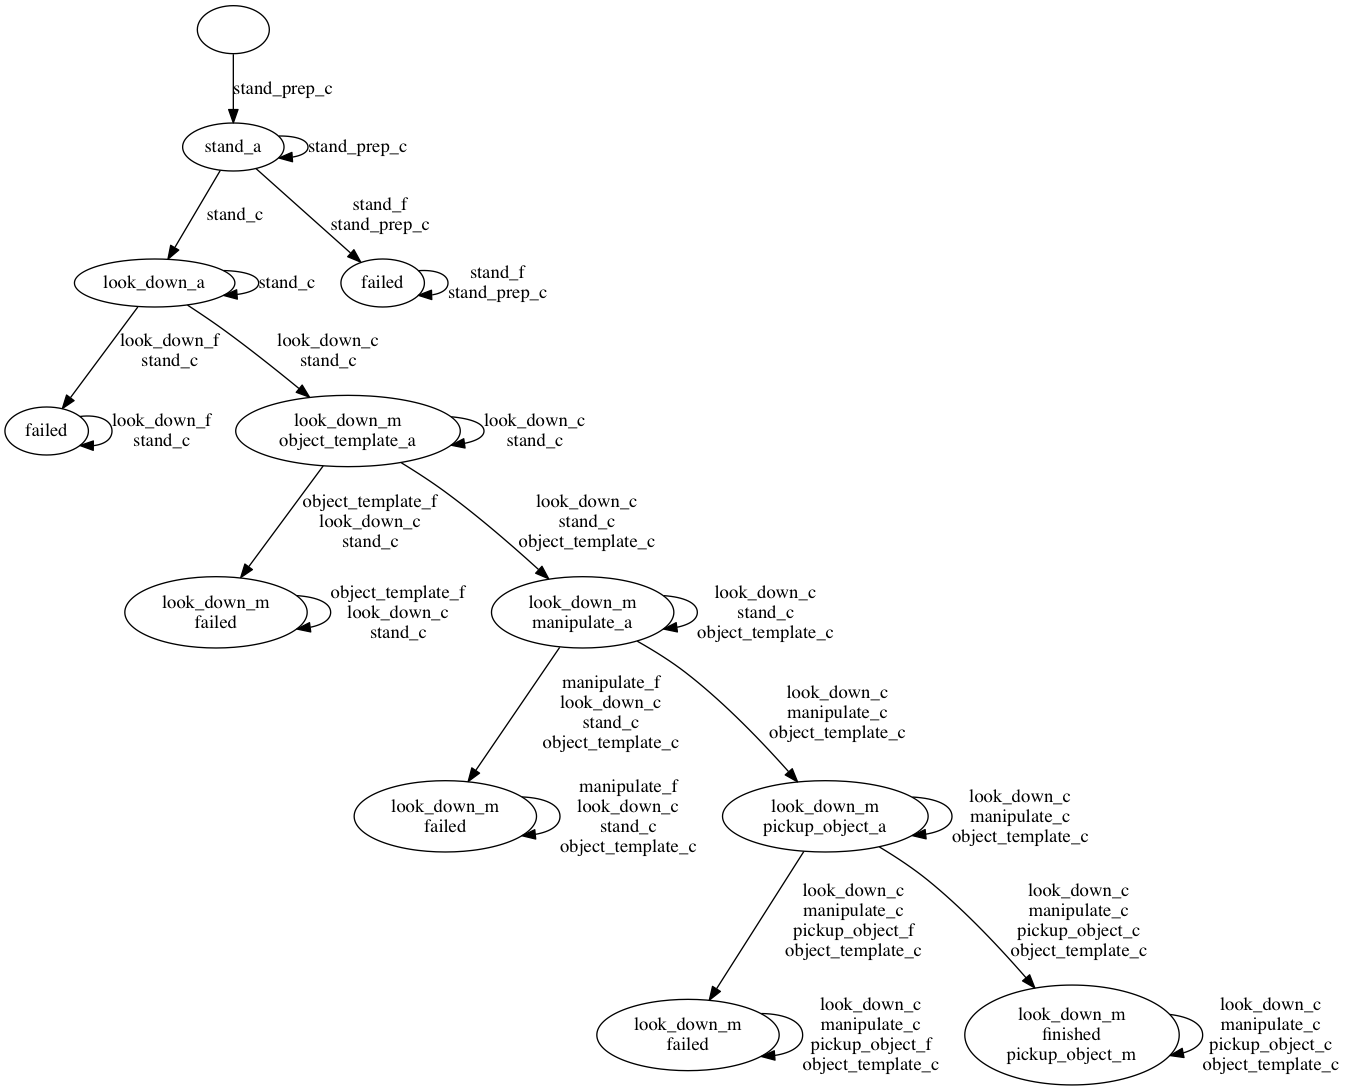
\includegraphics[width=0.95\columnwidth,clip]{./img/synthesized_automaton.png}
\caption{
	The output of \textsc{gr(1)} synthesis is a symbolic finite-state automaton.
	For clarity, only the atomic propositions that are $\True$ are depicted.
	The formal specification was generated from the user input $\mathcal{I} = \{ \mathtt{stand\_prep} \}$ and $\mathcal{G} = \{ \mathtt{pickup\_object} \}$, according to Section \ref{S:ltl}.
	\todo[inline, caption = {Finalize synthesized automaton figure}]{Replace with automaton that has memory propositions.}
}
\label{Fig:SynthesizedAutomaton}
\end{figure}

% END